\documentclass[11pt,a4paper]{article}

\usepackage[T1]{fontenc}
\usepackage[utf8]{inputenc}
\usepackage{lmodern}
\usepackage[margin=2.5cm]{geometry}
\usepackage{graphicx}
\usepackage{pdflscape}
\usepackage{float}
\usepackage{booktabs}
\usepackage{tabularx}
\usepackage{array}
\usepackage{xcolor}
\usepackage{listings}
\usepackage{caption}
\usepackage{enumitem}
\usepackage[hidelinks]{hyperref}

\definecolor{codebg}{RGB}{248,248,248}
\definecolor{kw}{RGB}{0,0,160}
\definecolor{cm}{RGB}{0,120,0}
\definecolor{st}{RGB}{163,21,21}

\lstset{
  language=C++,
  basicstyle=\ttfamily\footnotesize,
  keywordstyle=\color{kw}\bfseries,
  commentstyle=\color{cm}\itshape,
  stringstyle=\color{st},
  backgroundcolor=\color{codebg},
  frame=single,
  rulecolor=\color{black!25},
  breaklines=true,
  columns=fullflexible,
  keepspaces=true,
  showstringspaces=false,
  tabsize=4,
  morekeywords={override,constexpr,nullptr,noexcept,final,auto},
  xleftmargin=4pt,
  xrightmargin=4pt
}

\newcommand{\code}[1]{\texttt{#1}}
\newcolumntype{L}{>{\raggedright\arraybackslash}X}

\title{\textbf{Data Analytics Library in C++}\\[4pt]
\large An Object-Oriented Design Project}
\author{Chiraag K V, Vivek Reddy, Utkarsh Gupta, Russel Gandhi}
\date{October 2026}

\begin{document}

\maketitle

\begin{abstract}
This report presents a small data analytics library written in C++20. The library loads tabular data
from CSV files into typed columns, computes statistics (mean and median), filters rows using
composable condition objects, exports results to CSV and JSON, and renders scatter plots as SVG images.
The emphasis of the project is on \emph{object-oriented design}: the system is decomposed into
entities with single responsibilities that collaborate through abstract interfaces. The
implementation demonstrates inheritance, multiple and virtual inheritance, runtime polymorphism,
templates, a custom exception hierarchy, and automatic memory management with smart pointers.
\end{abstract}

\tableofcontents
\newpage

%=====================================================================
\section{Introduction}
%=====================================================================

A procedural approach to data analysis typically begins with free functions such as
\code{mean()}, \code{filter()} and \code{plot()}. While this works for small scripts, data and
behaviour remain loosely connected, and supporting a new data type, file format or statistic
requires changes in many places.

This project instead starts from the \emph{entities} in the problem domain, gives each one a
single responsibility, and connects them through abstract interfaces. New behaviour is added by
writing new classes rather than by modifying existing ones.

\subsection*{Objectives}
\begin{enumerate}[noitemsep]
  \item Store heterogeneous, typed columns in a single \code{DataSet}.
  \item Compute statistics through interchangeable algorithms.
  \item Filter rows with reusable, composable conditions.
  \item Import and export data in CSV and JSON formats.
  \item Produce a basic scatter-plot visualisation (SVG).
  \item Demonstrate core C++ OOP features and manage memory without manual \code{new}/\code{delete}.
\end{enumerate}

%=====================================================================
\section{Architecture Summary}
%=====================================================================

\subsection{Components}

The library is organised into three layers: a \textbf{core} that owns the data, a set of
\textbf{operations} that read the data but never own it, and an \textbf{I/O layer} that moves
data between files and memory. Table~\ref{tab:components} summarises the components.

\begin{table}[H]
\centering
\caption{Main components and their responsibilities}
\label{tab:components}
\begin{tabularx}{\textwidth}{@{}l L c l@{}}
\toprule
\textbf{Component} & \textbf{Responsibility} & \textbf{Owns data?} & \textbf{Files} \\
\midrule
\code{DataSet} & Central entity; holds a collection of columns & Yes & \code{DataSet.hpp/.cpp} \\
\code{ColumnBase}, \code{Column<T>} & A named, typed sequence of values & Yes & \code{ColumnBase.hpp}, \code{Column.hpp} \\
\code{Filter} & Applies a condition to a named column & No & \code{Filter.hpp/.cpp} \\
\code{Condition} \& subclasses & A test on a single value, combinable with And/Or/Not & No & \code{Condition.hpp/.cpp} \\
\code{IAnalyzer}, \code{StatisticsEngine} & Compute statistics (Strategy pattern) & No & \code{Analyzer.hpp/.cpp} \\
\code{IImporter}, \code{IExporter} & CSV and JSON input/output & No & \code{IO.hpp/.cpp} \\
\code{IVisualizer}, \code{ScatterPlot} & Render data as an SVG scatter plot & No & \code{Visualizer.hpp/.cpp} \\
\code{DataException} \& subclasses & Report errors by category & -- & \code{Exceptions.hpp} \\
\bottomrule
\end{tabularx}
\end{table}

\begin{figure}[H]
  \centering
  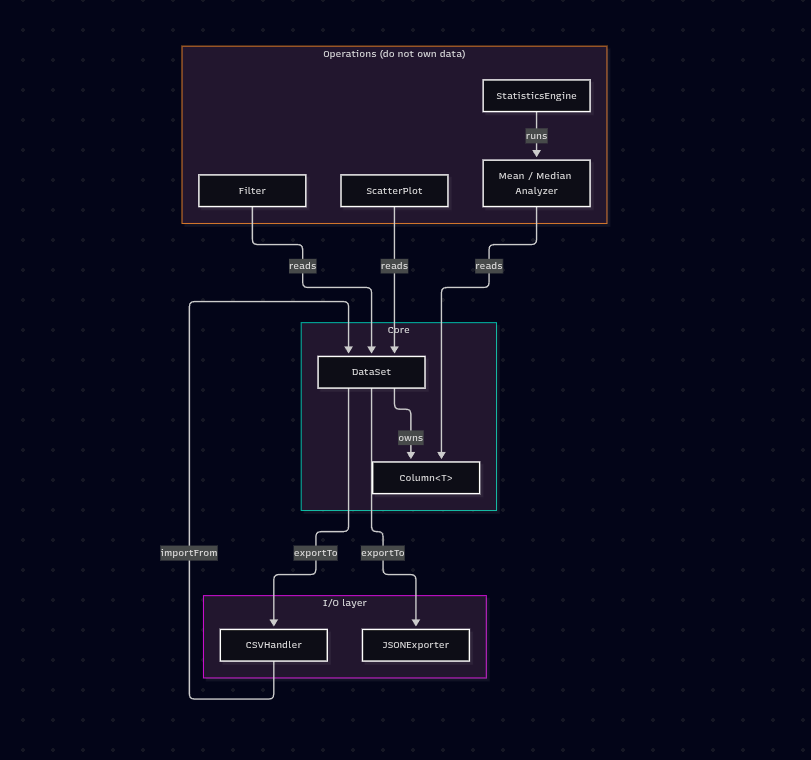
\includegraphics[width=0.72\textwidth,height=0.8\textheight,keepaspectratio]{supporting/flow.png}
  \caption{Layered architecture: operations read from the core; the I/O layer imports and exports it.}
  \label{fig:arch}
\end{figure}

\subsection{Data Flow}

Figure~\ref{fig:dataflow} shows the typical pipeline executed by the demo program. A CSV file is
imported into a \code{DataSet}; the data set is then analysed, plotted, and filtered, and the
filtered result is exported to CSV and JSON.

\begin{figure}[H]
  \centering
  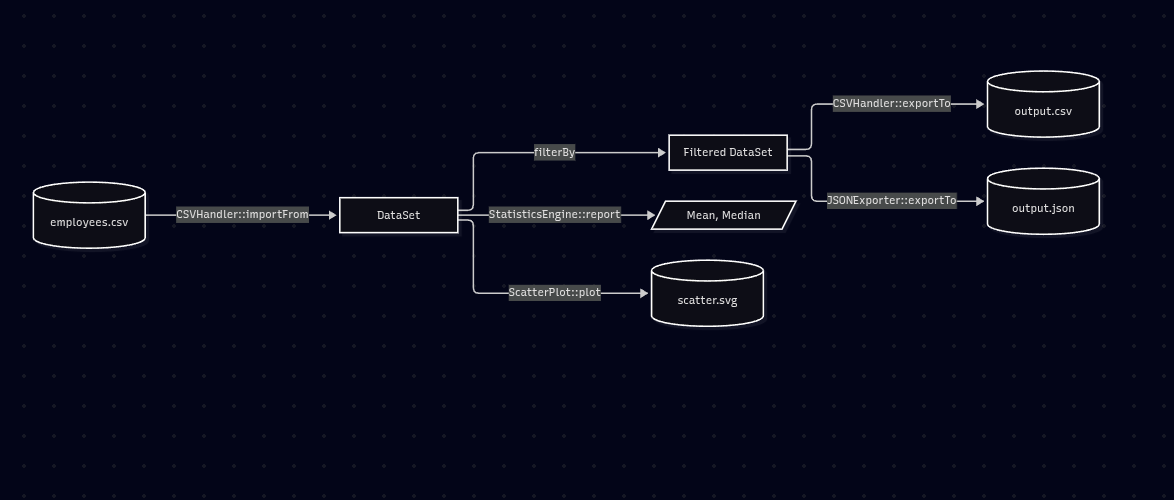
\includegraphics[width=\textwidth,height=0.8\textheight,keepaspectratio]{supporting/example.png}
  \caption{Data flow from CSV input to statistics, SVG plot and exported files.}
  \label{fig:dataflow}
\end{figure}

\subsection{Memory Ownership}

Ownership is expressed in the type system. A \code{DataSet} owns its columns and a
\code{StatisticsEngine} owns its analyzers through \code{std::unique\_ptr}. Conditions are the
one exception: they are immutable, so a \code{Filter} and any composite condition hold them
through \code{std::shared\_ptr}, which lets filters be copied and reused cheaply. All other access
is non-owning, through raw pointers or references (Figure~\ref{fig:memory}).

\begin{figure}[H]
  \centering
  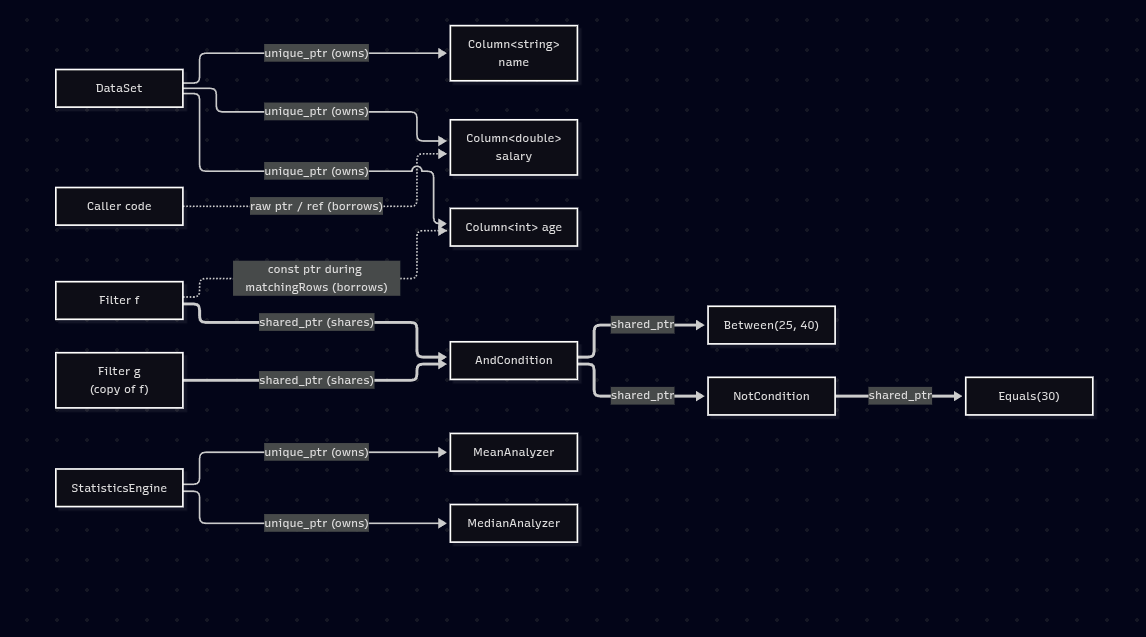
\includegraphics[width=0.9\textwidth,height=0.8\textheight,keepaspectratio]{supporting/memory.png}
  \caption{Ownership graph: solid arrows own (\code{unique\_ptr}), thick arrows share ownership (\code{shared\_ptr}), dotted arrows borrow.}
  \label{fig:memory}
\end{figure}

\subsection{Project Structure}

\begin{lstlisting}[language={},basicstyle=\ttfamily\small]
include/   Exceptions.hpp  ColumnBase.hpp  Column.hpp  Condition.hpp
           Filter.hpp      DataSet.hpp     Analyzer.hpp  IO.hpp
           Visualizer.hpp
src/       DataSet.cpp     Condition.cpp   Filter.cpp    Analyzer.cpp
           IO.cpp          Visualizer.cpp  main.cpp
data/      employees.csv
Makefile   (g++ -std=c++20 -Wall -Wextra -pedantic)
\end{lstlisting}

%=====================================================================
\section{Class Definitions}
%=====================================================================

The library's interface is spread over nine header files in \code{include/}. This section
describes what each header contains: its classes, their data members, and the role of each
important member function. Each module begins with its UML class diagram. In the diagrams,
\emph{italic} methods are pure virtual, \code{-} marks private members, \code{\#} marks protected
members, and \code{+} marks public members.

\begin{landscape}
\begin{figure}[H]
  \centering
  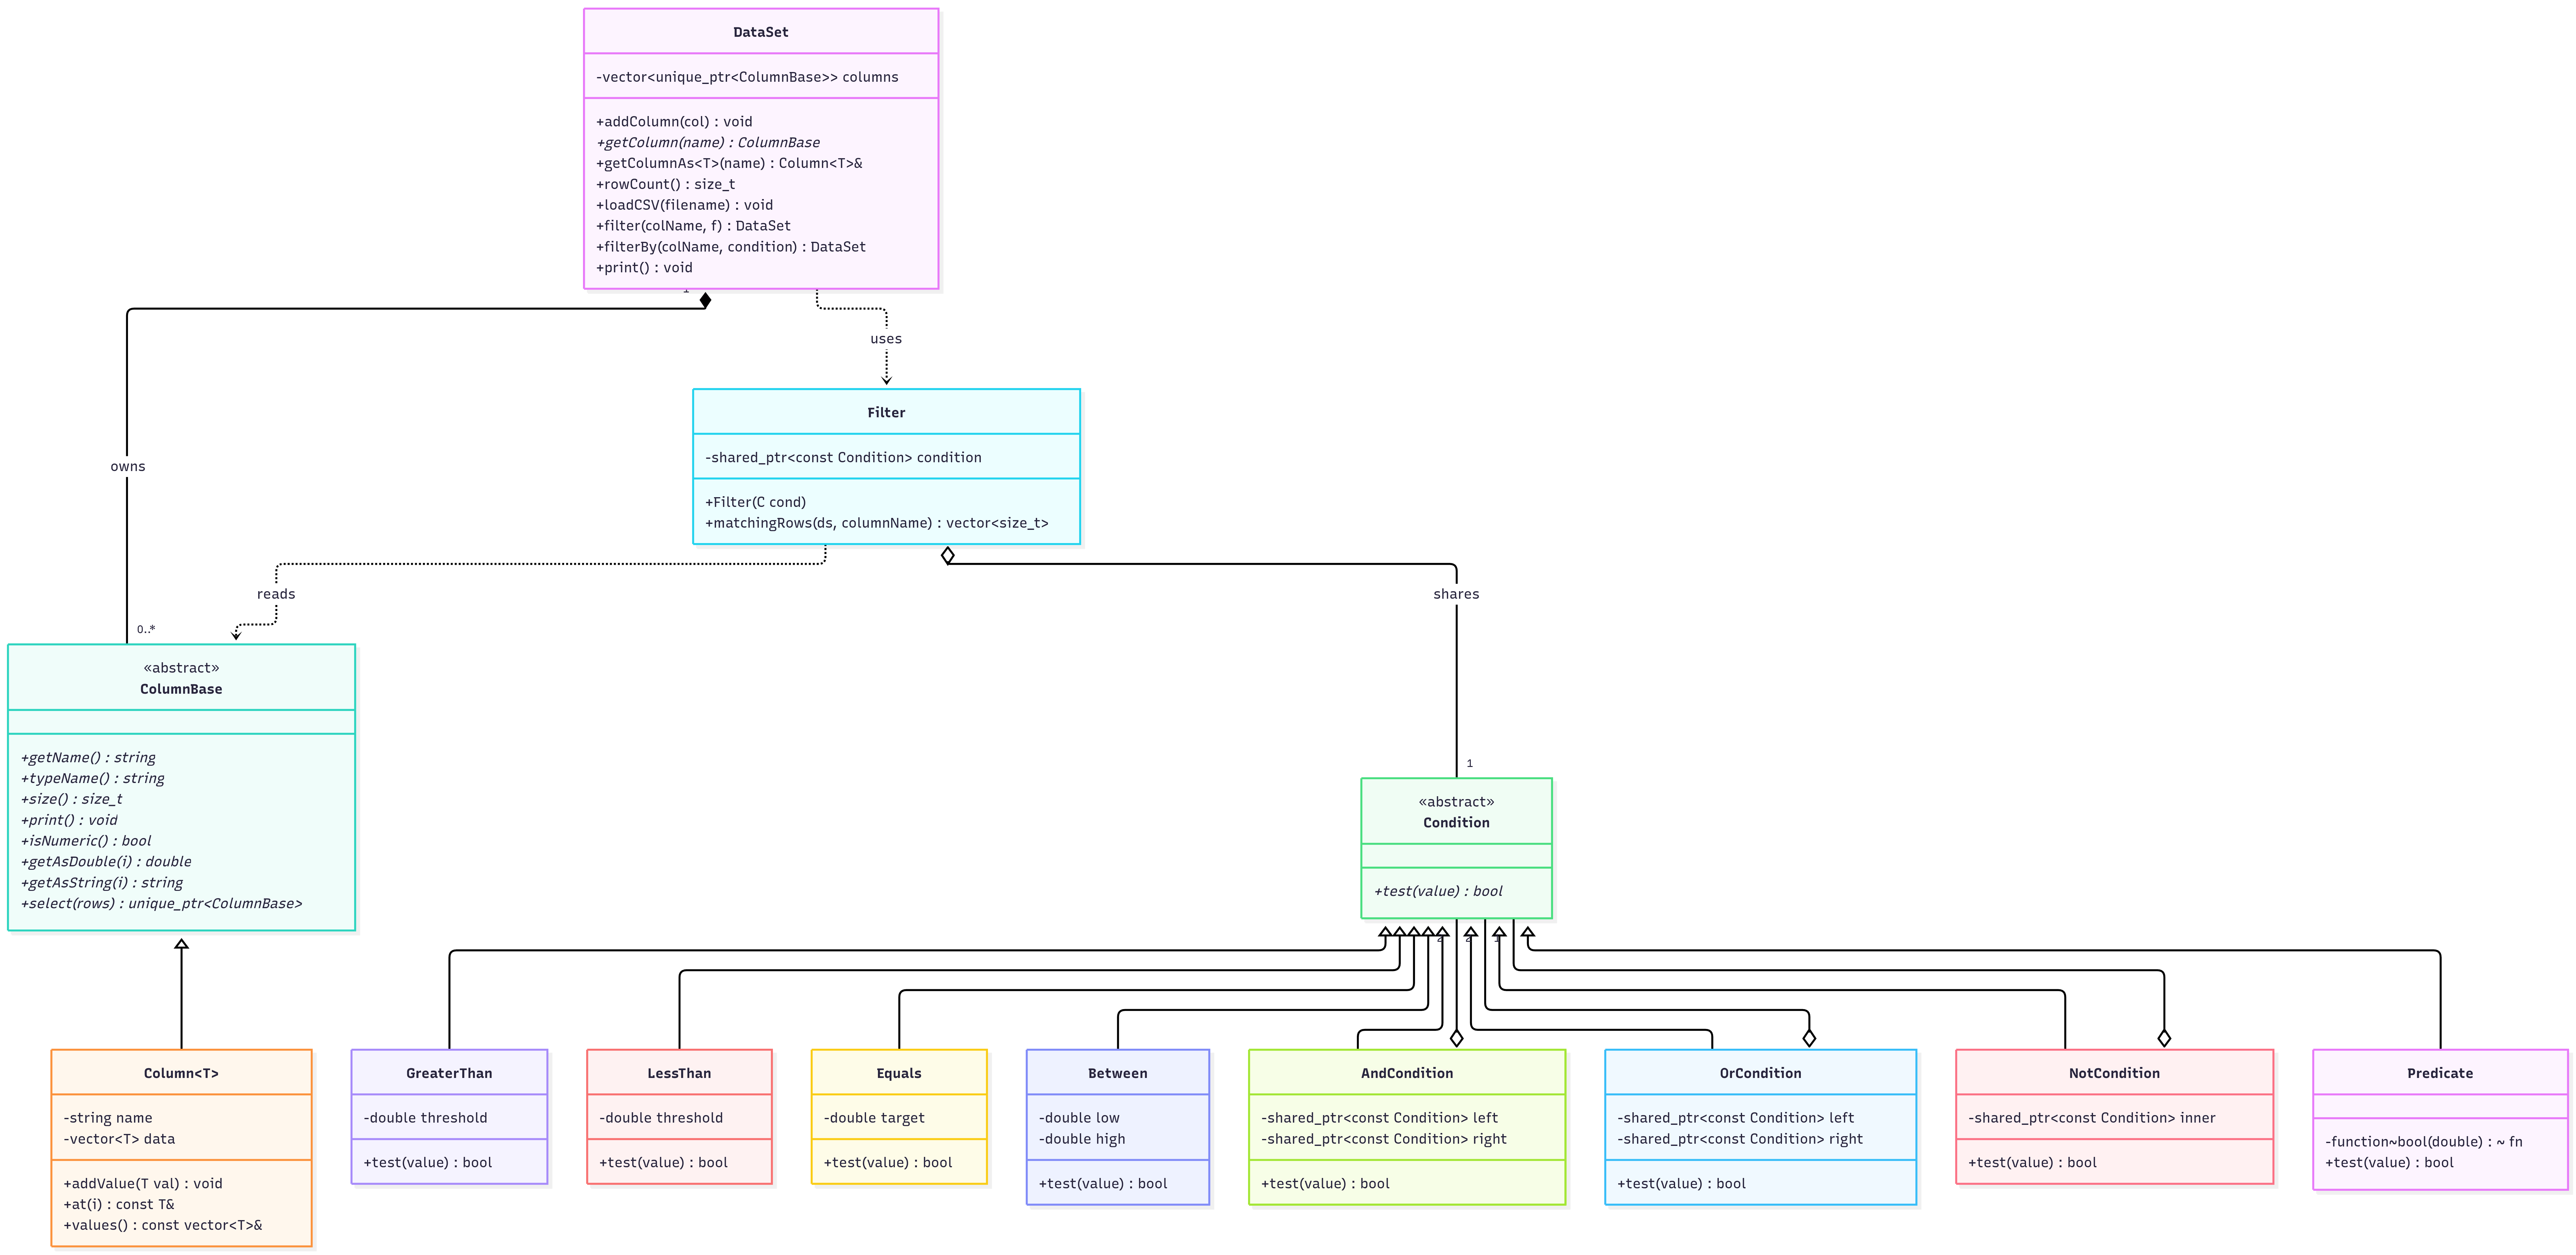
\includegraphics[width=\linewidth,height=0.85\textheight,keepaspectratio]{UML/DF.png}
  \caption{UML class diagram of the core package.}
  \label{fig:uml-core}
\end{figure}
\end{landscape}

\subsection{Core: DataSet, Columns, Filter and Conditions}

\subsubsection*{ColumnBase.hpp}

Declares \code{ColumnBase}, the abstract base class that every column implements. It holds no
data; it only defines what the rest of the library may ask of a column, without knowing the
column's value type. All of its functions are pure virtual, and it has a virtual destructor so that
columns can be safely destroyed through a base-class pointer.

\begin{description}[noitemsep,leftmargin=1.5em]
  \item[\code{getName()}, \code{typeName()}, \code{size()}] Return the column's name, its type as
    text (for example \code{"int"}), and its number of values.
  \item[\code{print()}] Writes the column's name, type and values to the console.
  \item[\code{isNumeric()}, \code{getAsDouble(i)}] Let analyzers, filters and the plotter treat any
    numeric column as a sequence of \code{double} values.
  \item[\code{getAsString(i)}] Returns one value as text; used by the CSV and JSON exporters.
  \item[\code{select(rows)}] Returns a new column containing only the given row indices; used by
    filtering.
\end{description}

\subsubsection*{Column.hpp}

Contains the class template \code{Column<T>}, the only concrete column type, together with the
helper trait \code{TypeName<T>}. Because it is a template, the whole implementation lives in the
header and there is no matching \code{.cpp} file.

\begin{description}[noitemsep,leftmargin=1.5em]
  \item[\code{TypeName<T>}] A small struct with specialisations for \code{int}, \code{double} and
    \code{string} that maps each type to a readable name; any other type is reported as
    \code{"unknown"}.
  \item[Data members] A private \code{name} and a private \code{vector<T> data} holding the values.
  \item[\code{addValue(val)}] Appends a value to the column.
  \item[\code{at(i)}, \code{values()}] Read access: \code{at} is bounds-checked and throws
    \code{std::out\_of\_range}; \code{values} returns a read-only reference to the whole vector.
  \item[Overrides] Implements every \code{ColumnBase} function. \code{getAsDouble} uses
    \code{if constexpr} so that numeric types are converted with \code{static\_cast} while
    \code{Column<string>} throws \code{TypeMismatchException}. \code{getAsString} returns strings
    unchanged and formats numbers with 15 significant digits.
\end{description}

\subsubsection*{DataSet.hpp}

Declares \code{DataSet}, the central entity of the library. Its only data member is a private
\code{vector<unique\_ptr<ColumnBase>>}, so it owns its columns and can store columns of different
types together. It can be moved but not copied, because \code{unique\_ptr} cannot be copied.

\begin{description}[noitemsep,leftmargin=1.5em]
  \item[\code{addColumn(col)}] Takes ownership of a column. Rejects null columns, duplicate names,
    and columns whose length differs from the existing ones.
  \item[\code{getColumn(name)}] Returns a non-owning pointer to a column, or throws
    \code{ColumnNotFoundException}. A \code{const} overload is provided.
  \item[\code{getColumnAs<T>(name)}] Member template that returns the column as a typed
    \code{Column<T>\&} using \code{dynamic\_cast}; throws \code{TypeMismatchException} if the
    column holds a different type.
  \item[\code{rowCount()}, \code{columnCount()}, \code{columnNames()}, \code{columnAt(i)}] Describe
    the data set's shape and give access to columns by position.
  \item[\code{loadCSV(filename)}] Replaces the contents with data read through \code{CSVHandler}.
  \item[\code{filter(colName, f)}] Returns a new \code{DataSet} containing only the rows whose
    value in \code{colName} satisfies the filter, for example
    \code{ds.filter("age", GreaterThan(30))}. The column is chosen here rather than when the
    filter is built, so one \code{Filter} can be reused on any data set or column.
  \item[\code{filterBy(colName, condition)}] Convenience overload for one-off conditions. It uses
    a C++20 \code{auto} parameter so any callable can be passed, and wraps it in a
    \code{Predicate}.
  \item[\code{print()}] Prints the data set's dimensions and every column.
\end{description}

\subsubsection*{Filter.hpp}

Declares \code{Filter}, which applies a \code{Condition} to a column. Its only data member is a
\code{shared\_ptr<const Condition>}. The constructor is a template constrained by the
\code{ConditionType} concept, so any \code{Condition} subclass can be passed by value and is
converted implicitly; this is what allows \code{ds.filter("age", GreaterThan(30))}. Its single
operation, \code{matchingRows(ds, columnName)}, checks that the column exists and is numeric, then
returns the indices of the rows for which the condition's \code{test} is true. \code{DataSet} is
only forward-declared here, which avoids a circular include between the two headers.

\subsubsection*{Condition.hpp}

Declares the abstract class \code{Condition} and its subclasses, arranged as a Composite
(Section~\ref{sec:composite}). \code{Condition} has a virtual destructor and one pure virtual
function, \code{test(value)}, which says whether a single \code{double} satisfies the condition.
The header also defines the concept \code{ConditionType}, which accepts any type derived from
\code{Condition}.

\begin{description}[noitemsep,leftmargin=1.5em]
  \item[\code{GreaterThan}, \code{LessThan}, \code{Equals}] Compare the value against a stored
    threshold or target.
  \item[\code{Between}] True when the value lies in the closed range $[\mathit{low}, \mathit{high}]$.
    The constructor throws \code{DataException} if \code{low > high}.
  \item[\code{AndCondition}, \code{OrCondition}] Hold two child conditions and combine their
    results with \code{\&\&} or \code{||}. Evaluation short-circuits.
  \item[\code{NotCondition}] Holds one child condition and negates it; for example
    \code{NotCondition(LessThan(30))} expresses ``at least 30''.
  \item[\code{Predicate}] Wraps a \code{function<bool(double)>} for conditions the classes above do
    not cover. The constructor rejects an empty function.
\end{description}

Composite conditions store their children as \code{shared\_ptr<const Condition>}, built from
concept-constrained template constructors, so they nest freely:
\begin{lstlisting}
Filter f = AndCondition(Between(25, 40), NotCondition(Equals(30)));
DataSet a = ds.filter("age", f);
DataSet b = other.filter("experience", f);   // same filter, different data
\end{lstlisting}

\subsection{Analytics: Strategy Pattern}

\begin{figure}[H]
  \centering
  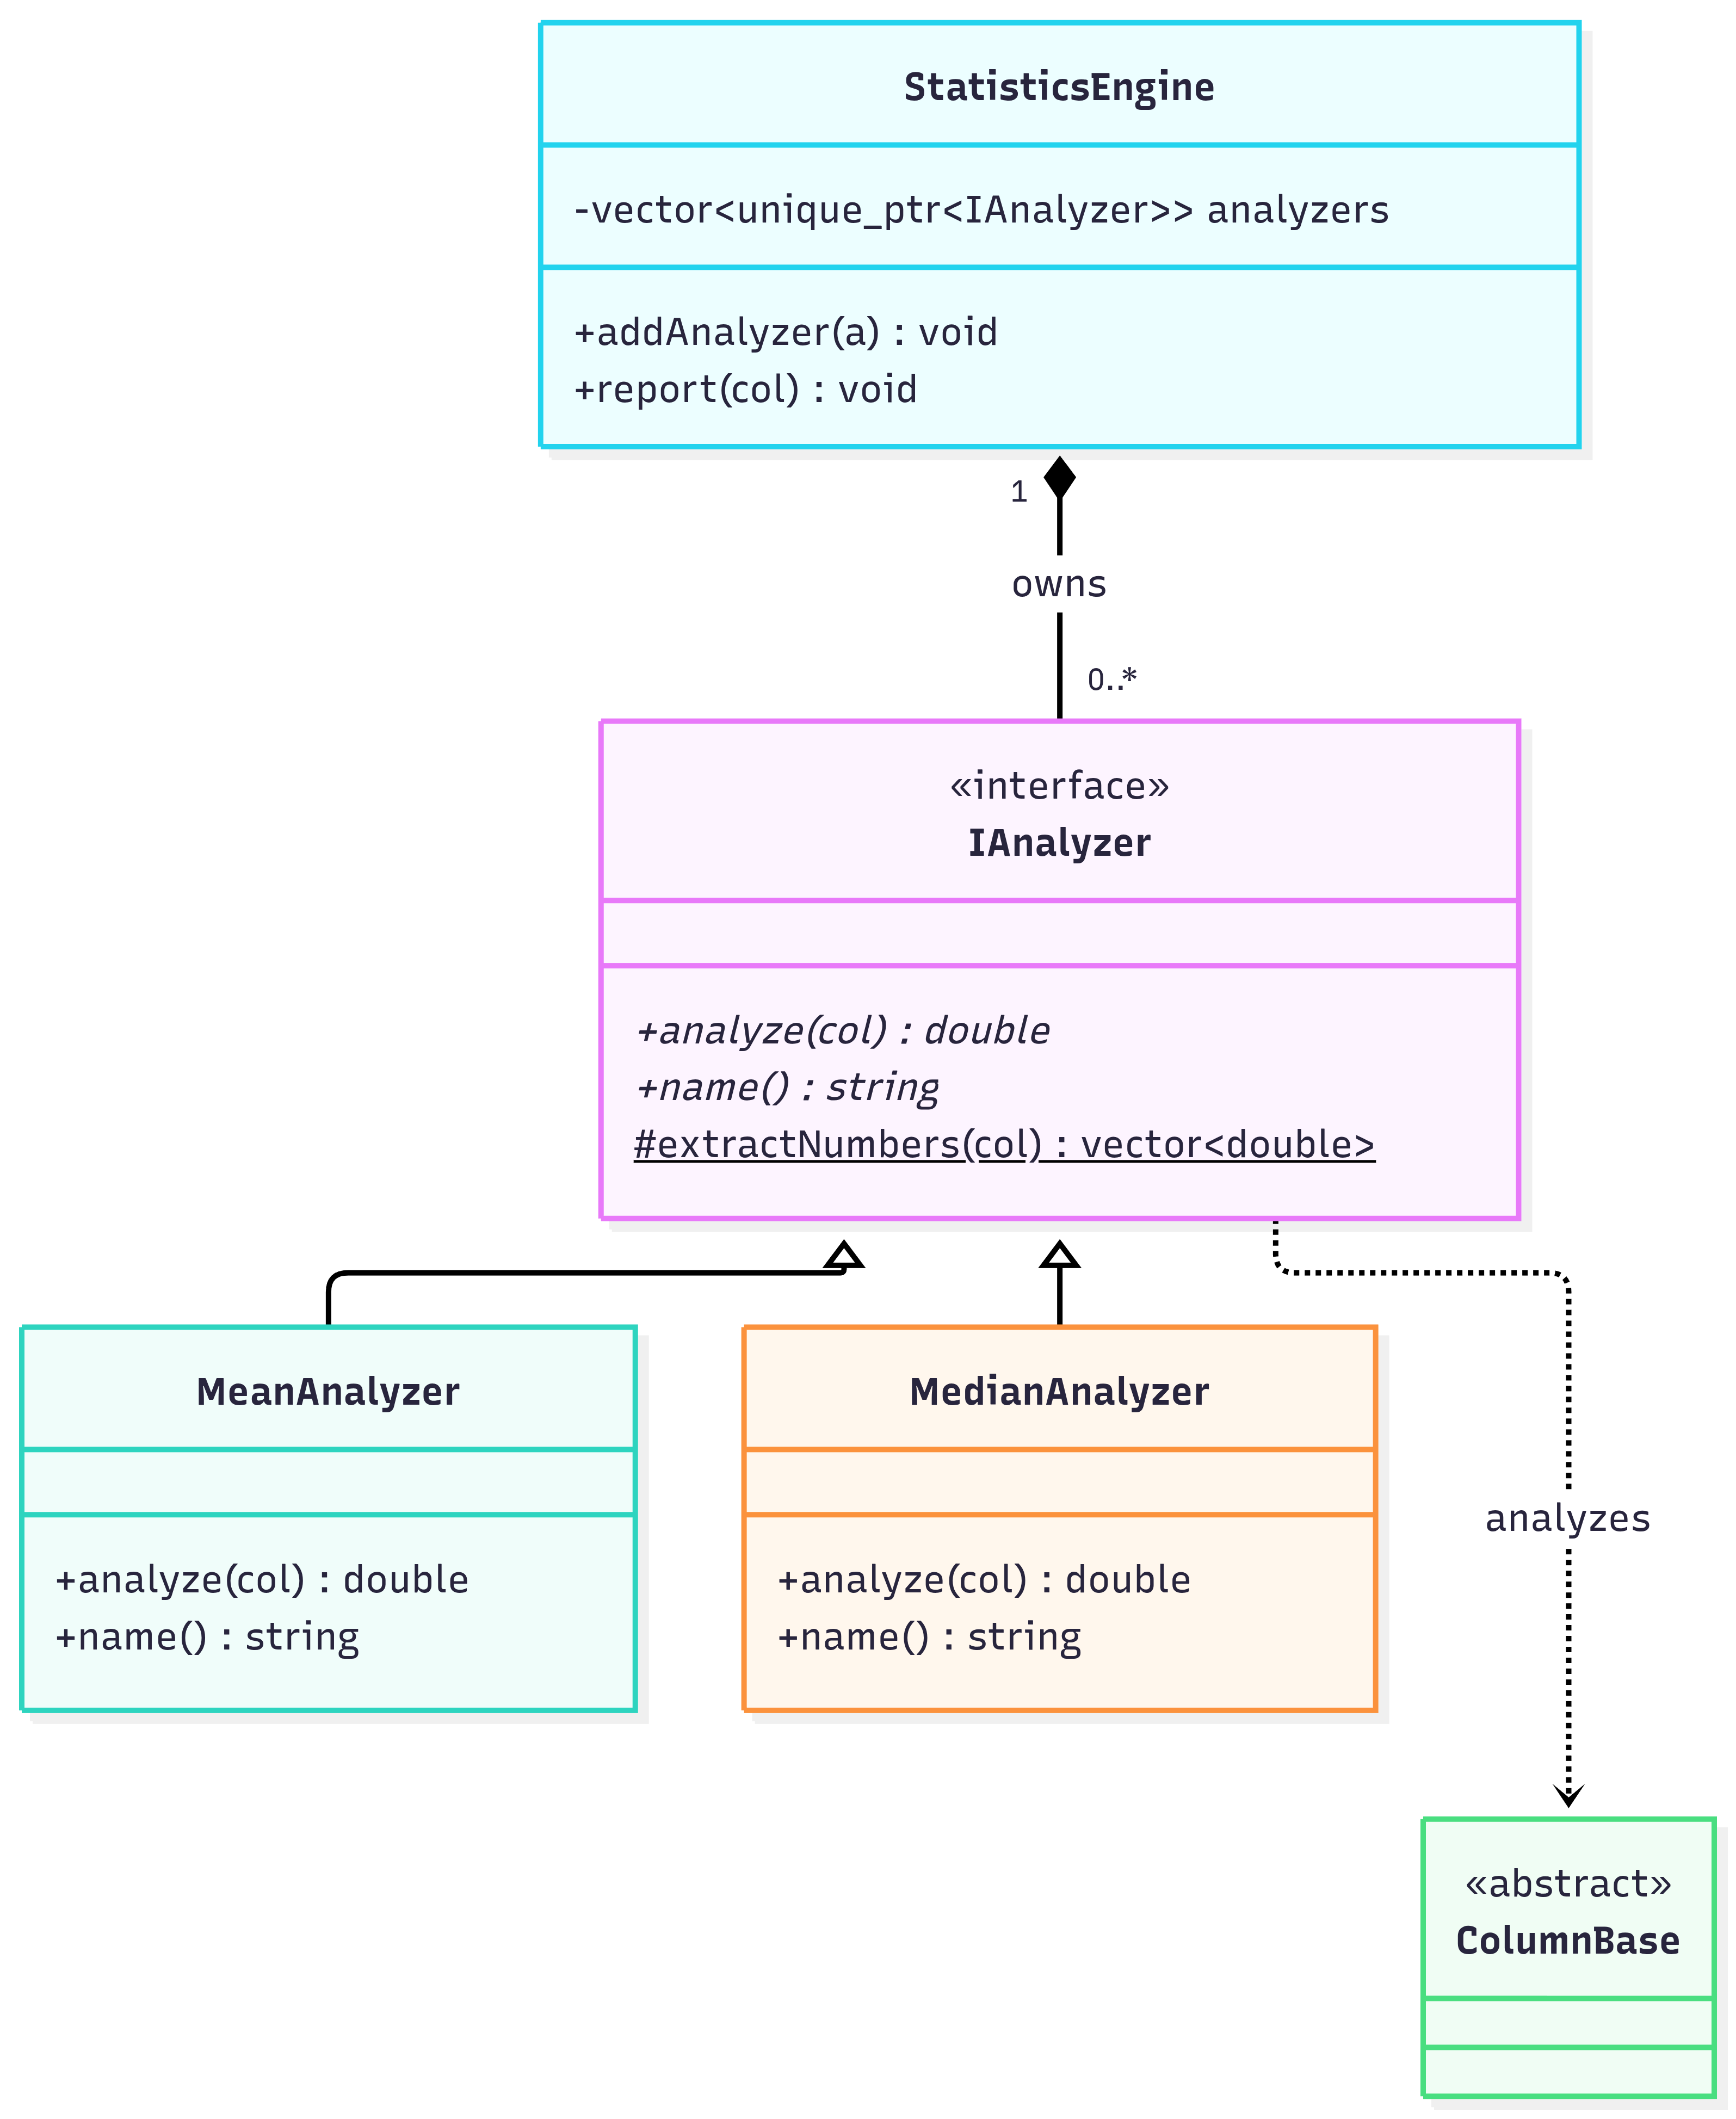
\includegraphics[width=0.62\textwidth,height=0.8\textheight,keepaspectratio]{UML/Analyser.png}
  \caption{UML class diagram of the analytics package.}
  \label{fig:uml-analytics}
\end{figure}

\subsubsection*{Analyzer.hpp}

Contains the analytics module, built on the Strategy pattern.

\begin{description}[noitemsep,leftmargin=1.5em]
  \item[\code{IAnalyzer}] Abstract strategy interface with two pure virtual functions:
    \code{analyze(col)}, which computes a single \code{double} from a column, and \code{name()},
    which returns the statistic's label. It also provides a protected static helper,
    \code{extractNumbers(col)}, which checks that the column is numeric and non-empty and copies
    its values into a \code{vector<double>}.
  \item[\code{MeanAnalyzer}] Concrete strategy that returns the arithmetic mean.
  \item[\code{MedianAnalyzer}] Concrete strategy that sorts the values and returns the middle value,
    or the average of the two middle values when the count is even.
  \item[\code{StatisticsEngine}] Owns a list of analyzers as \code{unique\_ptr<IAnalyzer>}.
    \code{addAnalyzer} registers a new strategy, and \code{report(col)} runs every registered
    strategy on a column and prints the results.
\end{description}

\subsection{I/O and Visualisation}

\begin{figure}[H]
  \centering
  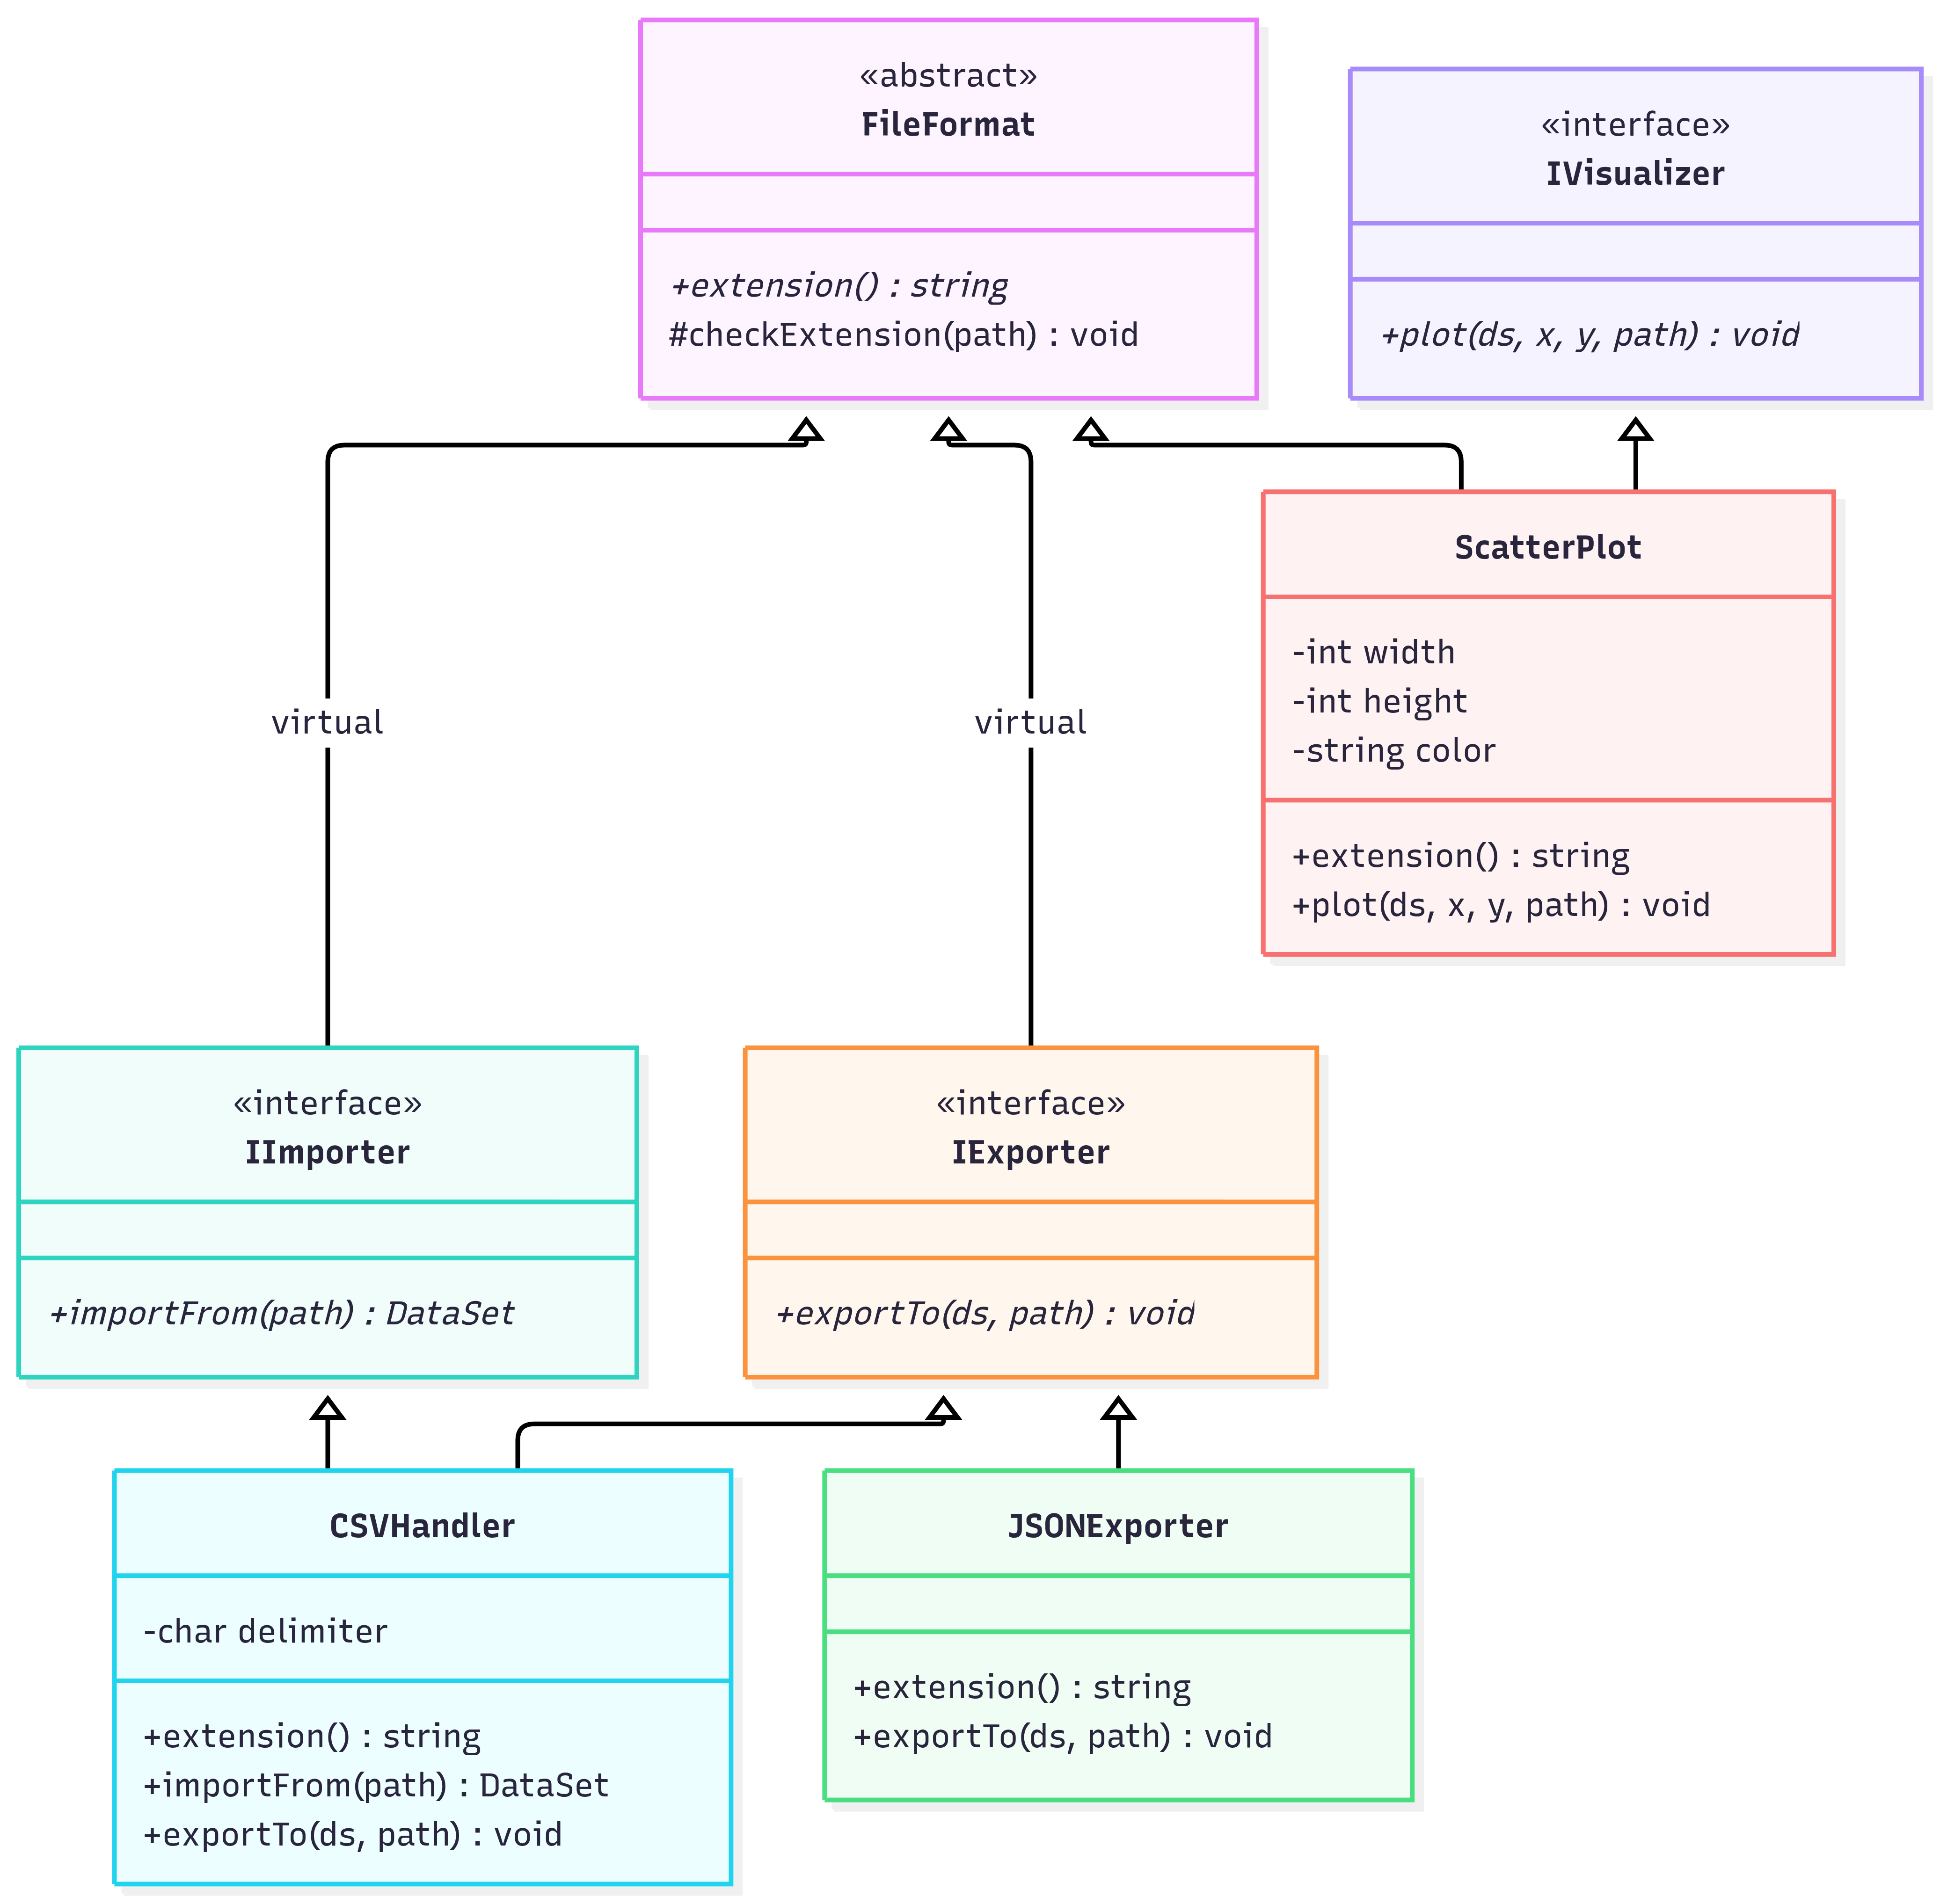
\includegraphics[width=0.85\textwidth,height=0.8\textheight,keepaspectratio]{UML/io.png}
  \caption{UML class diagram of the I/O and visualisation packages.}
  \label{fig:uml-io}
\end{figure}

\subsubsection*{IO.hpp}

Contains the file input/output classes, arranged as a diamond inheritance hierarchy.

\begin{description}[noitemsep,leftmargin=1.5em]
  \item[\code{FileFormat}] Abstract base for anything tied to a file type. It declares the pure
    virtual \code{extension()} (for example \code{".csv"}) and provides the protected helper
    \code{checkExtension(path)}, which throws \code{FileException} when a path has the wrong
    extension.
  \item[\code{IImporter}] Interface with \code{importFrom(path)}, which reads a file and returns a
    new \code{DataSet}. Inherits \code{FileFormat} \emph{virtually}.
  \item[\code{IExporter}] Interface with \code{exportTo(ds, path)}, which writes a \code{DataSet}
    to a file. Also inherits \code{FileFormat} \emph{virtually}.
  \item[\code{CSVHandler}] Inherits both \code{IImporter} and \code{IExporter}, so it can read and
    write CSV. It stores a configurable delimiter (a comma by default). On import it checks that
    every row has the right number of fields and infers each column's type as \code{int},
    \code{double} or \code{string}.
  \item[\code{JSONExporter}] Inherits only \code{IExporter}. Writes the data set as a JSON array
    of objects, with numbers unquoted and strings quoted and escaped.
\end{description}

\subsubsection*{Visualizer.hpp}

Contains the visualisation classes.

\begin{description}[noitemsep,leftmargin=1.5em]
  \item[\code{IVisualizer}] Interface with the pure virtual \code{plot(ds, xCol, yCol, path)},
    which renders two columns of a data set to a file.
  \item[\code{ScatterPlot}] Inherits both \code{IVisualizer} and \code{FileFormat}; its extension is
    \code{".svg"}, so the inherited \code{checkExtension} rejects other output paths. It stores the
    image width, height and point colour (by default $640 \times 480$ pixels in blue). The
    constructor rejects sizes too small to fit the axis margins. \code{plot} checks that both
    columns are numeric, scales the points to pixel coordinates, and writes an SVG file with grid
    lines, axis ticks and labels, a title, and a hover tooltip on every point.
\end{description}

\subsection{Exceptions}

\subsubsection*{Exceptions.hpp}

Defines the library's exception hierarchy. Every class is a few lines long, so the file has no
matching \code{.cpp}. Each constructor builds a descriptive message from its arguments.

\begin{description}[noitemsep,leftmargin=1.5em]
  \item[\code{DataException}] Base of all library errors; derives from \code{std::runtime\_error}
    and reuses its constructors. Also thrown directly for general rule violations such as a
    duplicate column name.
  \item[\code{ColumnNotFoundException}] Takes the missing column's name.
  \item[\code{TypeMismatchException}] Takes the column name and the expected type, for example
    \code{"numeric"}.
  \item[\code{EmptyDataException}] Signals that there is no data to work on.
  \item[\code{FileException}] Signals file problems: a missing or unwritable file, a wrong
    extension, or a malformed CSV row.
\end{description}

%=====================================================================
\section{Usage of OOP Concepts}
%=====================================================================

Table~\ref{tab:oop} maps each concept to where it is used; the subsections below explain each one
with a short excerpt from the code.

\begin{table}[H]
\centering
\caption{OOP concepts and where they appear}
\label{tab:oop}
\begin{tabularx}{\textwidth}{@{}l L@{}}
\toprule
\textbf{Concept} & \textbf{Usage in the project} \\
\midrule
Abstraction & Pure virtual interfaces \code{ColumnBase}, \code{Condition}, \code{IAnalyzer}, \code{FileFormat}, \code{IImporter}, \code{IExporter}, \code{IVisualizer} \\
Encapsulation & Private column data and column list; \code{addColumn} enforces invariants \\
Inheritance & \code{Column<T>}, condition classes, analyzers, exporters, \code{ScatterPlot}, exception classes \\
Multiple inheritance & \code{CSVHandler : IImporter, IExporter}; \code{ScatterPlot : IVisualizer, FileFormat} \\
Virtual inheritance & \code{IImporter} and \code{IExporter} inherit \code{virtual FileFormat} \\
Runtime polymorphism & Heterogeneous \code{vector<unique\_ptr<ColumnBase>>}; \code{Condition::test} calls from \code{Filter}; analyzer, exporter and visualiser calls through base references \\
Templates & \code{Column<T>}, \code{TypeName<T>} specialisation, \code{if constexpr}, \code{getColumnAs<T>()}, \code{auto} parameter, \code{ConditionType} concept \\
Exception handling & \code{DataException} hierarchy; catch by \code{const} reference \\
Smart pointers & \code{unique\_ptr} and \code{make\_unique} throughout; \code{shared\_ptr} for immutable conditions; move-only \code{DataSet} \\
Design patterns & Strategy pattern for analyzers; Composite pattern for conditions \\
\bottomrule
\end{tabularx}
\end{table}

\subsection{Abstraction}

Interfaces declare \emph{what} an object can do without specifying \emph{how}. A class with at
least one pure virtual function (\code{= 0}) cannot be instantiated:

\begin{lstlisting}
class IAnalyzer {
public:
    virtual ~IAnalyzer() = default;
    virtual double analyze(const ColumnBase& col) const = 0;
    virtual string name() const = 0;
};
\end{lstlisting}

The rest of the library (filters, analyzers, exporters, the plotter) depends only on such
interfaces, never on concrete column types. Likewise, \code{Filter} only calls
\code{Condition::test} and never knows which kind of condition it holds.

\subsection{Encapsulation}

Each column's values are private and modified only through \code{addValue}; reads go through the
bounds-checked \code{at()}. \code{DataSet::addColumn} protects the data set's invariants:

\begin{lstlisting}
void DataSet::addColumn(unique_ptr<ColumnBase> col) {
    if (!col) throw DataException("Cannot add a null column");
    for (const auto& c : columns)
        if (c->getName() == col->getName())
            throw DataException("Duplicate column name: " + col->getName());
    if (!columns.empty() && col->size() != rowCount())
        throw DataException(/* row count mismatch */);
    columns.push_back(move(col));
}
\end{lstlisting}

\code{IAnalyzer::extractNumbers} is \code{protected}: a helper for subclasses, hidden from users.

\subsection{Inheritance}

\begin{itemize}[noitemsep]
  \item \code{Column<T>} inherits \code{ColumnBase}.
  \item \code{MeanAnalyzer} and \code{MedianAnalyzer} inherit \code{IAnalyzer}.
  \item \code{CSVHandler}, \code{JSONExporter} and \code{ScatterPlot} inherit their interfaces.
  \item All custom exceptions inherit \code{DataException}, which inherits \code{std::runtime\_error}.
\end{itemize}

\subsection{Multiple and Virtual Inheritance}

\code{CSVHandler} can both read and write CSV, so it inherits from both \code{IImporter} and
\code{IExporter}. Both interfaces derive from \code{FileFormat}, forming a \emph{diamond}:

\begin{lstlisting}
class FileFormat { public: virtual string extension() const = 0; /* ... */ };
class IImporter : public virtual FileFormat { /* ... */ };
class IExporter : public virtual FileFormat { /* ... */ };
class CSVHandler : public IImporter, public IExporter { /* ... */ };
\end{lstlisting}

Without the \code{virtual} keyword, \code{CSVHandler} would contain two \code{FileFormat}
sub-objects and calls to \code{extension()} would be ambiguous. Virtual inheritance ensures a
single shared base, overridden once. \code{ScatterPlot} uses ordinary multiple inheritance from
\code{IVisualizer} and \code{FileFormat} to reuse the extension check for \code{.svg} files.

\subsection{Runtime Polymorphism}

A single container holds columns of different concrete types; each call is dispatched through the
virtual table to the correct implementation:

\begin{lstlisting}
vector<unique_ptr<ColumnBase>> columns;   // Column<int>, Column<double>, Column<string>

for (const auto& c : columns) c->print(); // calls Column<T>::print for each T
\end{lstlisting}

The same mechanism runs every analyzer in \code{StatisticsEngine::report}, every exporter in the
demo's export loop, and the plotter through an \code{IVisualizer\&}. Every polymorphic base declares a
\textbf{virtual destructor} so that deleting through a base pointer destroys the derived object
correctly, and every override is marked \code{override} so that signature mistakes are compile-time
errors.

\subsection{Templates}

\paragraph{Class template.} \code{Column<T>} is written once and instantiated for \code{int},
\code{double} and \code{string}. Being a template, it is defined entirely in its header.

\paragraph{Template specialisation.} A trait maps each type to a readable name:
\begin{lstlisting}
template <typename T> struct TypeName    { static string get() { return "unknown"; } };
template <> struct TypeName<int>         { static string get() { return "int"; } };
template <> struct TypeName<double>      { static string get() { return "double"; } };
\end{lstlisting}

\paragraph{Compile-time branching.} \code{if constexpr} compiles only the branch valid for
\code{T}, so a string column never attempts a numeric cast:
\begin{lstlisting}
double getAsDouble(size_t i) const override {
    if constexpr (is_arithmetic_v<T>)
        return static_cast<double>(at(i));
    else
        throw TypeMismatchException(name, "numeric");
}
\end{lstlisting}

\paragraph{Member and abbreviated function templates.} \code{getColumnAs<T>()} returns a typed
reference using \code{dynamic\_cast}, and \code{filterBy} uses a C++20 \code{auto} parameter to
accept any callable:
\begin{lstlisting}
auto& ages = ds.getColumnAs<int>("age");
DataSet even = ds.filterBy("age", [](double a) { return (int)a % 2 == 0; });
\end{lstlisting}

\paragraph{Concepts.} The C++20 concept \code{ConditionType} restricts the constructor templates
of \code{Filter} and the composite conditions to types derived from \code{Condition}. Passing
anything else is rejected at compile time with a readable error, instead of failing deep inside
\code{make\_shared}:
\begin{lstlisting}
template <typename C>
concept ConditionType = derived_from<C, Condition>;

template <ConditionType C>
Filter(C cond) : condition(make_shared<C>(move(cond))) {}
\end{lstlisting}

\subsection{Exception Handling}

All library errors derive from \code{DataException}, allowing callers to catch errors at the level
of detail they need:

\begin{lstlisting}
try {
    MeanAnalyzer().analyze(*ds.getColumn("name"));
} catch (const TypeMismatchException& e) {   // most specific
    cout << e.what() << "\n";
} catch (const DataException& e) {           // any library error
    cerr << e.what() << "\n";
} catch (const exception& e) {               // anything else
    cerr << e.what() << "\n";
}
\end{lstlisting}

\begin{table}[H]
\centering
\caption{Exception types and when they are thrown}
\begin{tabularx}{\textwidth}{@{}l L@{}}
\toprule
\textbf{Exception} & \textbf{Thrown when} \\
\midrule
\code{ColumnNotFoundException} & A column name does not exist \\
\code{TypeMismatchException} & A numeric operation is applied to a string column, or \code{getColumnAs<T>} uses the wrong \code{T} \\
\code{EmptyDataException} & Analysing an empty column or plotting no rows \\
\code{FileException} & File missing or unwritable, wrong extension, malformed CSV row \\
\code{DataException} & Duplicate column, row-count mismatch, null column or analyzer \\
\bottomrule
\end{tabularx}
\end{table}

\subsection{Smart Pointers and Memory Management}

The code contains no \code{new} or \code{delete}. Objects are created with \code{make\_unique}
and ownership transfer is explicit through \code{move}:

\begin{lstlisting}
auto col = make_unique<Column<double>>("score");
col->addValue(9.5);
ds.addColumn(move(col));   // ownership passes to the DataSet
\end{lstlisting}

Because \code{unique\_ptr} cannot be copied, \code{DataSet} is \emph{move-only}; functions such as
\code{filter()} return a new \code{DataSet} by value, which is moved rather than copied.

Conditions use \code{shared\_ptr<const Condition>} instead. They never change after construction,
so sharing them is safe, and it makes \code{Filter} and the composite conditions cheap to copy: a
copy shares the same condition tree rather than duplicating it.

\subsection{Design Patterns}

\subsubsection*{Strategy}

Each analyzer is an interchangeable strategy. Adding a new statistic, such as standard deviation,
requires only one new class overriding \code{analyze()}; no existing class changes, in line with
the Open/Closed Principle.

\begin{lstlisting}
StatisticsEngine engine;
engine.addAnalyzer(make_unique<MeanAnalyzer>());
engine.addAnalyzer(make_unique<MedianAnalyzer>());
engine.report(*ds.getColumn("salary"));
\end{lstlisting}

\subsubsection*{Composite}
\label{sec:composite}

Conditions follow the Composite pattern. Simple conditions (\code{GreaterThan}, \code{Between},
\ldots) are leaves; \code{AndCondition}, \code{OrCondition} and \code{NotCondition} are composites
that hold other conditions and are themselves conditions. Clients treat both the same way, by
calling \code{test()}, so arbitrarily nested expressions can be built without changing
\code{Filter}. A new kind of condition only needs a new subclass that overrides \code{test()}.

\begin{lstlisting}
// 25 <= age <= 40, excluding 30, or anyone over 55
Filter f = OrCondition(AndCondition(Between(25, 40), NotCondition(Equals(30))),
                       GreaterThan(55));
\end{lstlisting}

%=====================================================================
\section{Results}
%=====================================================================

The demo program (\code{src/main.cpp}) exercises every feature on a sample of ten employees.
CSV type inference correctly produced \code{string} columns for \emph{name} and
\emph{department}, \code{int} columns for \emph{age} and \emph{experience}, and a \code{double}
column for \emph{salary}.

\begin{table}[H]
\centering
\caption{Statistics computed by \code{StatisticsEngine}}
\begin{tabular}{@{}lrr@{}}
\toprule
\textbf{Column} & \textbf{Mean} & \textbf{Median} \\
\midrule
salary & 78700.1 & 75500.2 \\
age & 33.5 & 32 \\
\bottomrule
\end{tabular}
\end{table}

Filtering the \emph{age} column with \code{GreaterThan(30)} returned 6 of the 10 rows, which were exported to
\code{output.csv} and \code{output.json}. Every deliberate error case (missing column, numeric
operation on a string column, wrong typed access, missing file, wrong plot extension, duplicate
column) raised the expected exception. The project compiles without warnings under
\code{-Wall -Wextra -pedantic}.

\begin{figure}[H]
  \centering
  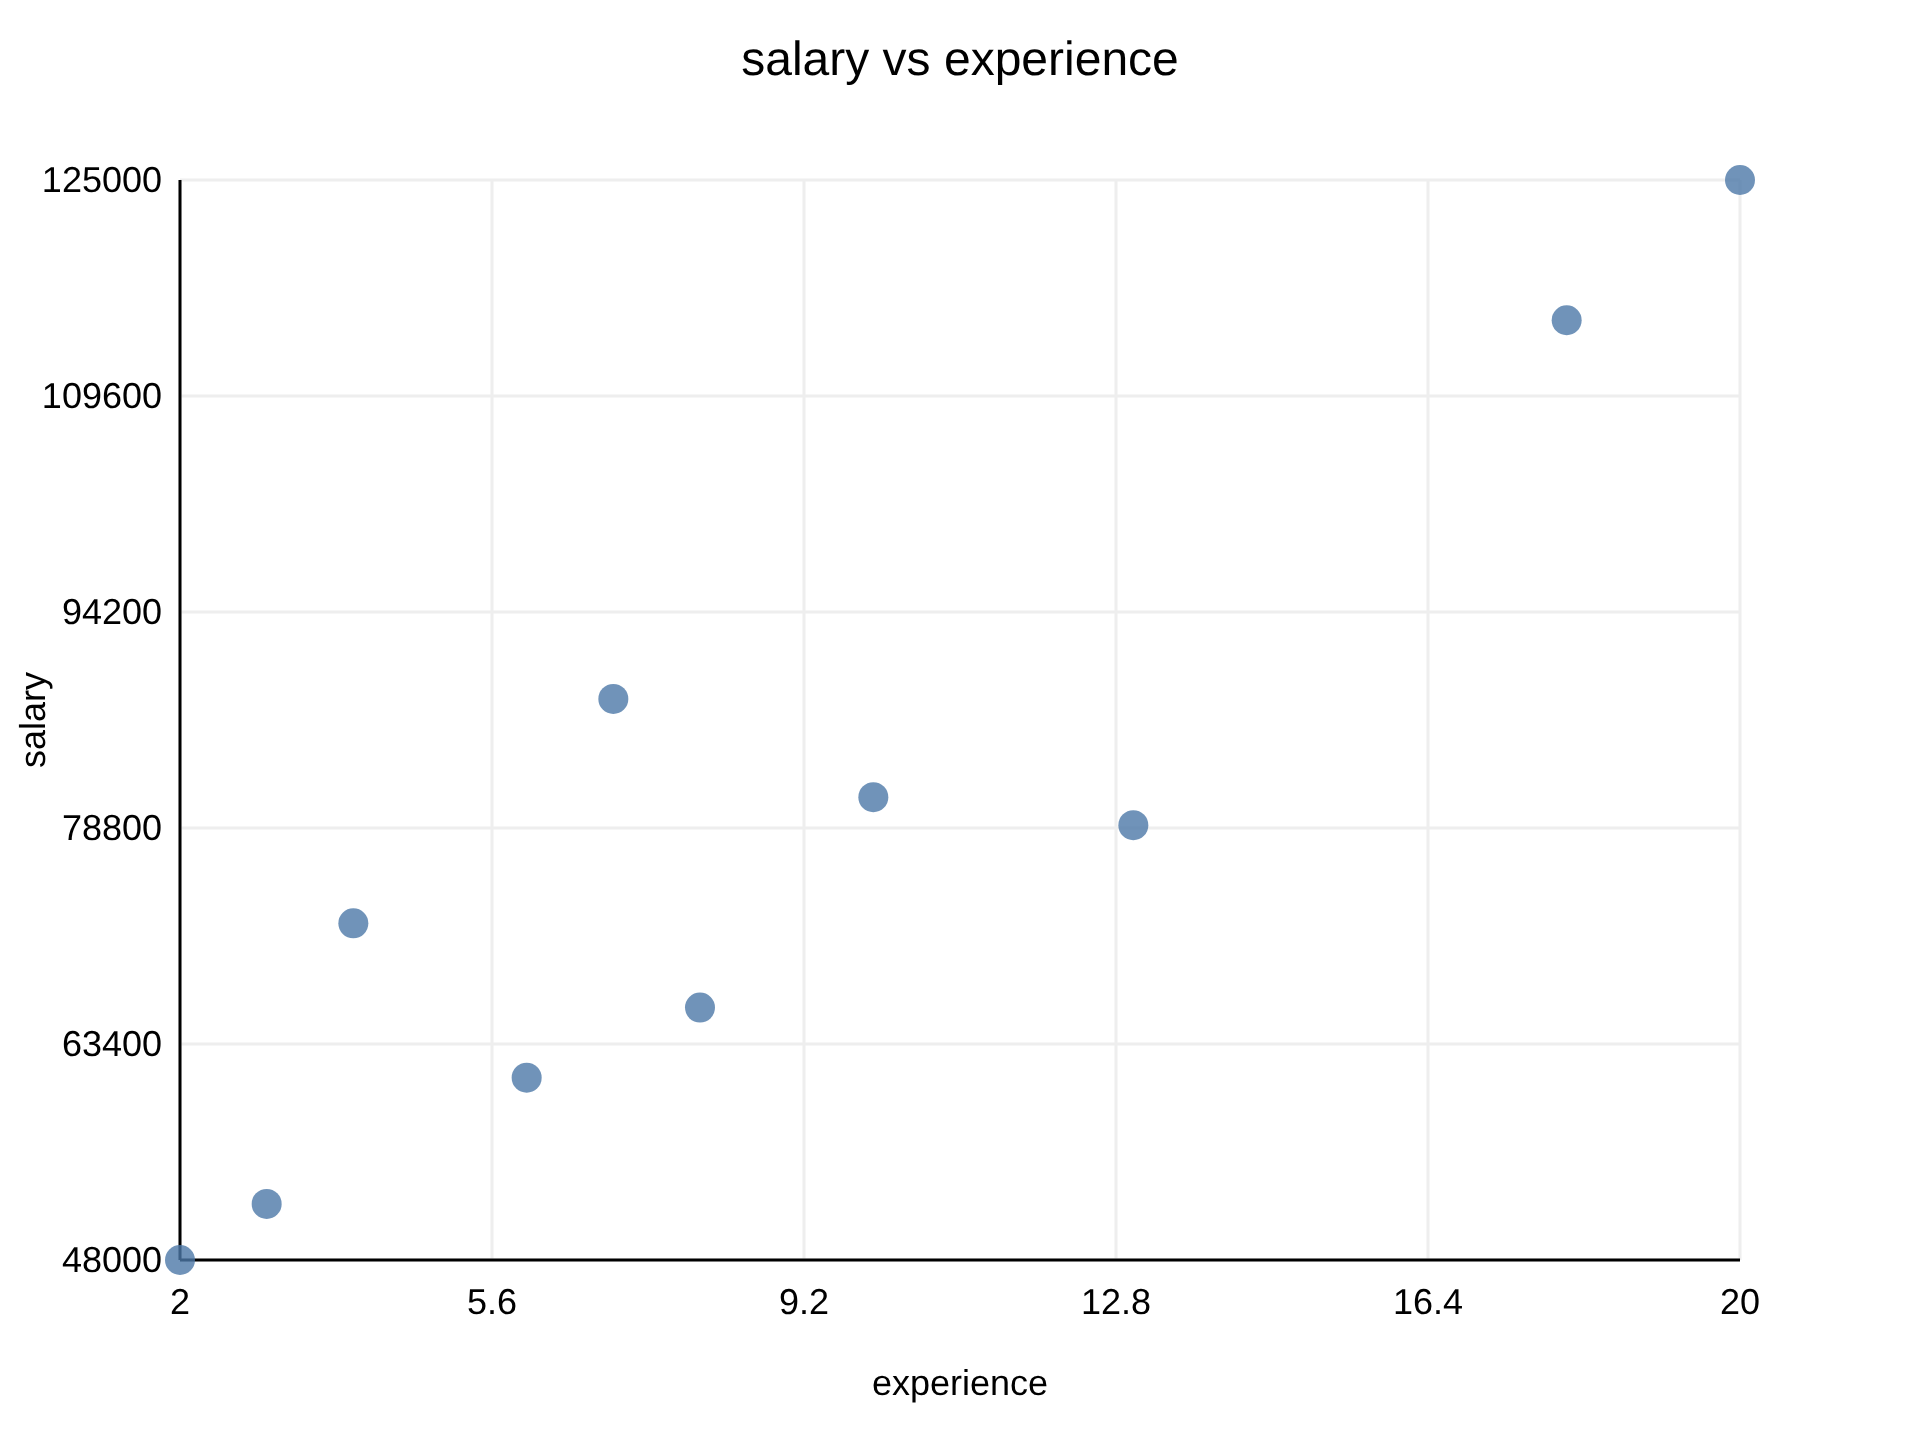
\includegraphics[width=0.75\textwidth,height=0.8\textheight,keepaspectratio]{supporting/scatter.png}
  \caption{SVG scatter plot of salary against experience, produced by \code{ScatterPlot}.}
  \label{fig:scatter}
\end{figure}

%=====================================================================
\section{Conclusion}
%=====================================================================

Designing around entities and interfaces rather than free functions produced a library that is
easy to extend and safe to use. New statistics, file formats and chart types can each be added as a
single new class without modifying existing code, and filter conditions can be combined freely
through the Composite pattern. Smart pointers eliminate manual memory
management, and the exception hierarchy makes failures explicit and easy to handle.

\paragraph{Limitations and future work.} Filters currently support only numeric columns, the CSV
parser does not handle quoted fields, and JSON is export-only. Additional analyzers (standard
deviation, correlation), chart types (line, bar) and conditions can be added by subclassing
\code{IAnalyzer}, \code{IVisualizer} and \code{Condition}.

\begin{thebibliography}{9}
\bibitem{stroustrup} B.~Stroustrup, \emph{The C++ Programming Language}, 4th ed. Addison-Wesley, 2013.
\bibitem{cppref} cppreference.com, \emph{C++ Reference}. \url{https://en.cppreference.com}
\end{thebibliography}

\end{document}
